\documentclass[tikz,border=6pt]{standalone}
\usepackage{tikz}
\usepackage{amsmath,amssymb}
\usepackage{xcolor}
\usetikzlibrary{arrows.meta,positioning,shapes.geometric,backgrounds,fit,calc,decorations.pathmorphing,shadows}

% ---- palette ----
\definecolor{packBG}{HTML}{DBEAFE}
\definecolor{packAccent}{HTML}{2563EB}
\definecolor{casRed}{HTML}{DC2626}
\definecolor{txtBG}{HTML}{DCFCE7}
\definecolor{txtAccent}{HTML}{059669}
\definecolor{imgBG}{HTML}{FED7AA}
\definecolor{imgAccent}{HTML}{EA580C}
\definecolor{howPurple}{HTML}{7C3AED}
\definecolor{anchorBG}{HTML}{E0E7FF}
\definecolor{hybridBG}{HTML}{EDE9FE}
\definecolor{railA}{HTML}{FCA5A5}
\definecolor{railB}{HTML}{FCD34D}
\definecolor{railC}{HTML}{86EFAC}
\definecolor{railD}{HTML}{93C5FD}
\definecolor{greyLine}{HTML}{4B5563}

\begin{document}
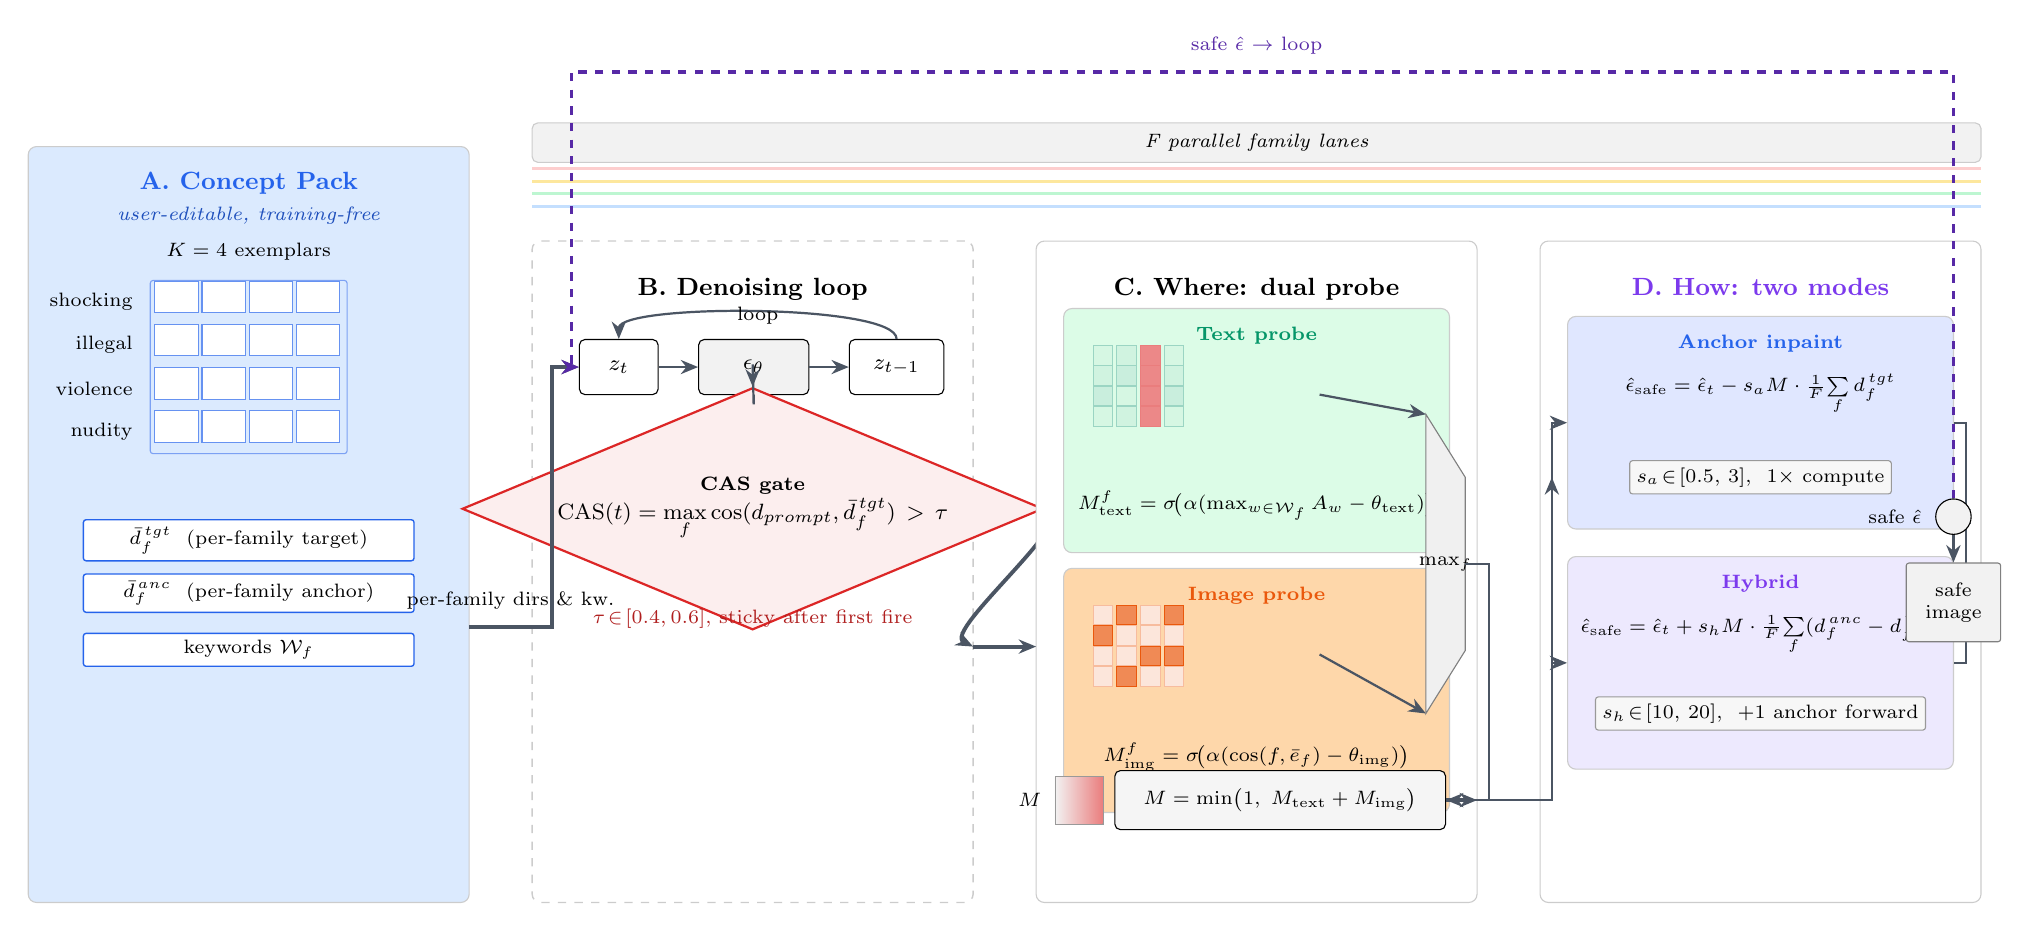
\begin{tikzpicture}[
    font=\footnotesize,
    >={Stealth[length=2.2mm,width=1.8mm]},
    thin,
    arrw/.style={->, line width=0.8pt, draw=greyLine},
    bigarrow/.style={->, line width=1.4pt, draw=greyLine},
    thumb/.style={draw=packAccent!70,line width=0.4pt,fill=white,minimum width=5.5mm,minimum height=4mm,inner sep=0pt},
    chip/.style={draw=packAccent,line width=0.5pt,fill=white,rounded corners=1pt,inner sep=2.5pt,font=\scriptsize},
    tag/.style={draw=black!40,fill=black!3,rounded corners=1pt,inner sep=2.5pt,font=\scriptsize},
    stageTitle/.style={font=\small\bfseries},
    colBG/.style={rounded corners=3pt,draw=black!20,line width=0.4pt},
]

% ============== LAYOUT CONSTANTS ==============
% total width ~ 24cm, height ~11cm
\def\colW{5.6}     % column width
\def\colWin{4.9}   % inner box width
\def\gap{0.8}      % gap between columns

% column x-centers
\pgfmathsetmacro{\Ax}{0}
\pgfmathsetmacro{\Bx}{\Ax + \colW + \gap}
\pgfmathsetmacro{\Cx}{\Bx + \colW + \gap}
\pgfmathsetmacro{\Dx}{\Cx + \colW + \gap}

% ============== TOP BANNER (across B-D) ==============
\pgfmathsetmacro{\bannerW}{\Dx + \colW/2 - (\Bx - \colW/2)}
\node[fill=black!5,draw=black!20,rounded corners=2pt,inner sep=2pt,
      minimum width=\bannerW cm,
      minimum height=5mm,
      anchor=center,font=\scriptsize\itshape]
      (banner) at ($(\Bx - \colW/2, 4.85)!0.5!(\Dx + \colW/2, 4.85)$) {F parallel family lanes};

% four faint rails beneath banner spanning B-D
\foreach \i/\c in {0/railA,1/railB,2/railC,3/railD} {
  \pgfmathsetmacro{\yr}{4.52 - 0.16*\i}
  \draw[\c,line width=1.2pt,opacity=0.55]
    (\Bx - \colW/2, \yr) -- (\Dx + \colW/2, \yr);
}

% ============== COLUMN A : CONCEPT PACK ==============
\node[colBG,fill=packBG,minimum width=\colW cm,minimum height=9.6cm,anchor=center]
     (colA) at (\Ax,0) {};
\node[stageTitle,anchor=north,text=packAccent] at (\Ax,4.6) {A.~Concept Pack};
\node[font=\scriptsize\itshape,anchor=north,text=packAccent!80!black] at (\Ax,4.15) {user-editable, training-free};

% K=4 exemplars caption
\node[font=\scriptsize,anchor=north] at (\Ax, 3.7) {$K=4$ exemplars};

% 4x4 thumbnail grid
\def\gridX{\Ax - 1.25}
\def\gridY{3.25}
\foreach \r/\lab in {0/shocking,1/illegal,2/violence,3/nudity} {
  \node[anchor=east,font=\scriptsize] at (\gridX - 0.1, \gridY - 0.42 - 0.55*\r) {\lab};
  \foreach \c in {0,1,2,3} {
    \pgfmathsetmacro{\tx}{\gridX + 0.05 + 0.6*\c}
    \pgfmathsetmacro{\ty}{\gridY - 0.15 - 0.55*\r}
    \node[thumb,anchor=north west] at (\tx,\ty) {};
  }
}
\draw[packAccent!60,line width=0.4pt,rounded corners=1pt]
  (\gridX, \gridY - 2.35) rectangle (\gridX + 2.5, \gridY - 0.15);

% two stacked vector chips + keywords chip
\node[chip,minimum width=4.2cm,anchor=center] (dtgt) at (\Ax, -0.2)
   {$\bar d^{\,tgt}_f$ \ (per-family target)};
\node[chip,minimum width=4.2cm,anchor=center,below=1.5mm of dtgt] (danc)
   {$\bar d^{\,anc}_f$ \ (per-family anchor)};
\node[chip,minimum width=4.2cm,anchor=center,below=2.5mm of danc] (kw)
   {keywords $\mathcal{W}_f$};

% exit arrow right (to column B) -- label LIFTED above the arrow
\coordinate (Aexit) at (\Ax + \colW/2, -1.3);

% ============== COLUMN B : DENOISING LOOP ==============
\node[colBG,dashed,line width=0.5pt,fill=white,
      minimum width=\colW cm,minimum height=8.4cm,anchor=center]
     (colB) at (\Bx,-0.6) {};
\node[stageTitle,anchor=north] at (\Bx,3.25) {B.~Denoising loop};

% self-loop: z_t -> eps_theta -> z_{t-1}
\node[draw,rounded corners=2pt,fill=white,minimum width=1.0cm,minimum height=0.7cm]
     (zt) at (\Bx - 1.7, 2.0) {$z_t$};
\node[draw,rounded corners=2pt,fill=black!5,minimum width=1.4cm,minimum height=0.7cm,right=5mm of zt]
     (eps) {$\epsilon_\theta$};
\node[draw,rounded corners=2pt,fill=white,minimum width=1.2cm,minimum height=0.7cm,right=5mm of eps]
     (ztm) {$z_{t-1}$};
\draw[arrw] (zt) -- (eps);
\draw[arrw] (eps) -- (ztm);
% loop back -- lowered peak so doesn't touch column title (was 0.7, now 0.45)
\draw[arrw] (ztm.north) .. controls +(0,0.45) and +(0,0.45) .. (zt.north);
\node[font=\scriptsize,anchor=south] at ($(zt)!0.5!(ztm)+(0,0.42)$) {loop};

% CAS diamond (red)
\node[diamond,draw=casRed,line width=0.8pt,fill=casRed!8,aspect=2.4,
      inner sep=2pt,minimum width=4.8cm,minimum height=1.9cm,
      align=center]
     (cas) at (\Bx, 0.2)
     {\scriptsize\textbf{CAS gate}\\[1pt]
      $\displaystyle \mathrm{CAS}(t)=\max_f \cos(d_{prompt},\bar d^{\,tgt}_f)\,>\,\tau$};
\node[font=\scriptsize,anchor=north,text=casRed!80!black] at (\Bx, -0.95)
     {$\tau\!\in\![0.4,0.6]$, sticky after first fire};

% epsilon feeds into CAS
\draw[arrw] (eps.south) .. controls +(0,-0.5) and +(0,0.7) .. (cas.north);

% fire exit -- label repositioned away from arrow
\coordinate (Bexit) at (\Bx + \colW/2, -1.55);
\draw[bigarrow] (cas.east) .. controls +(0.6,0) and +(-0.4,0.2) .. (Bexit);
\node[font=\scriptsize,text=txtAccent!60!black,anchor=west]
     at ($(cas.east)+(0.15,-0.32)$) {\checkmark\ fire};

% A -> B : single unified arrow (no double arrowhead)
\draw[bigarrow] (Aexit) -- (\Bx - \colW/2 + 0.25, -1.3)
  -- (\Bx - \colW/2 + 0.25, 2.0) -- (zt.west);
% label LIFTED
\node[font=\scriptsize,anchor=south,align=center]
  at ($(Aexit)!0.5!(\Bx - \colW/2 + 0.25, -1.3)+(0,0.1)$) {per-family dirs \& kw.};

% ============== COLUMN C : DUAL PROBE ==============
\node[colBG,fill=white,minimum width=\colW cm,minimum height=8.4cm,anchor=center]
     (colC) at (\Cx,-0.6) {};
\node[stageTitle,anchor=north] at (\Cx,3.25) {C.~Where: dual probe};

% --- TOP sub-row: Text probe (box height 3.1cm, spans y=-0.35..2.75) ---
\node[colBG,fill=txtBG,minimum width=\colWin cm,minimum height=3.1cm,anchor=north]
     (txtBox) at (\Cx, 2.75) {};
\node[anchor=north,font=\scriptsize\bfseries,text=txtAccent] at (\Cx,2.63) {Text probe};

% stylized 4x4 cross-attention heatmap (one column red) -- upper half of box
\def\tmX{\Cx - 1.95}
\def\tmY{2.15}
\foreach \r in {0,1,2,3} {
  \foreach \c in {0,1,2,3} {
    \pgfmathsetmacro{\tx}{\tmX + 0.30*\c}
    \pgfmathsetmacro{\ty}{\tmY - 0.26*\r}
    \pgfmathtruncatemacro{\isRed}{(\c==2)?1:0}
    \ifnum\isRed=1
      \node[draw=casRed!60,fill=casRed!55,minimum size=2.5mm,inner sep=0pt] at (\tx,\ty) {};
    \else
      \pgfmathsetmacro{\opa}{0.15 + 0.15*mod(\r+\c,3)}
      \node[draw=txtAccent!40,fill=txtAccent!30,fill opacity=\opa,minimum size=2.5mm,inner sep=0pt] at (\tx,\ty) {};
    \fi
  }
}
% formula BELOW the grid (was overlapping at y=2.1; now at y=0.55)
\node[anchor=north,font=\scriptsize] at (\Cx, 0.55)
  {$M^f_{\mathrm{text}} = \sigma\!\big(\alpha(\textstyle\max_{w\in\mathcal{W}_f} A_w - \theta_{\mathrm{text}})\big)$};

% --- BOTTOM sub-row: Image probe (box height 3.1cm, spans y=-3.65..-0.55) ---
\node[colBG,fill=imgBG,minimum width=\colWin cm,minimum height=3.1cm,anchor=north]
     (imgBox) at (\Cx, -0.55) {};
\node[anchor=north,font=\scriptsize\bfseries,text=imgAccent] at (\Cx,-0.67) {Image probe};

% CLIP-feature 4x4 grid with scattered orange -- upper half of box
\def\imX{\Cx - 1.95}
\def\imY{-1.15}
\foreach \r in {0,1,2,3} {
  \foreach \c in {0,1,2,3} {
    \pgfmathsetmacro{\tx}{\imX + 0.30*\c}
    \pgfmathsetmacro{\ty}{\imY - 0.26*\r}
    \node[draw=imgAccent!40,fill=imgAccent!15,minimum size=2.5mm,inner sep=0pt] at (\tx,\ty) {};
  }
}
\foreach \r/\cc in {0/1,0/3,1/0,2/2,2/3,3/1} {
  \pgfmathsetmacro{\tx}{\imX + 0.30*\cc}
  \pgfmathsetmacro{\ty}{\imY - 0.26*\r}
  \node[draw=imgAccent,fill=imgAccent!70,minimum size=2.5mm,inner sep=0pt] at (\tx,\ty) {};
}
% formula BELOW the image grid (was overlapping at y=-1.2; now at y=-2.65)
\node[anchor=north,font=\scriptsize] at (\Cx, -2.65)
  {$M^f_{\mathrm{img}} = \sigma\!\big(\alpha(\cos(f,\bar e_f) - \theta_{\mathrm{img}})\big)$};

% max_f converging funnel (right side, between both sub-rows)
\coordinate (funTopL) at (\Cx + \colW/2 - 0.65, 1.4);
\coordinate (funTopR) at (\Cx + \colW/2 - 0.15, 0.6);
\coordinate (funBotL) at (\Cx + \colW/2 - 0.65, -2.4);
\coordinate (funBotR) at (\Cx + \colW/2 - 0.15, -1.6);
\draw[draw=black!50,fill=black!6,line width=0.4pt]
  (funTopL) -- (funTopR) -- (funBotR) -- (funBotL) -- cycle;
\node[font=\scriptsize] at (\Cx + \colW/2 - 0.4, -0.5) {$\max_f$};

% fusion box at the bottom of column C
\node[draw,rounded corners=2pt,fill=black!4,line width=0.4pt,
      minimum width=4.2cm,minimum height=0.75cm,anchor=center,font=\scriptsize]
     (fuse) at (\Cx + 0.3, -3.5)
     {$M = \min\!\big(1,\; M_{\mathrm{text}} + M_{\mathrm{img}}\big)$};

% connect text/img grid CENTERS to funnel entrance, then funnel -> fuse
\draw[arrw] (\Cx + 0.8, 1.65) -- (funTopL);
\draw[arrw] (\Cx + 0.8, -1.65) -- (funBotL);
\draw[arrw] ($(funTopR)!0.5!(funBotR)$) -- ++(0.3,0) |- (fuse.east);

% small mask thumbnail next to fusion box label
\node[draw=black!40,line width=0.3pt,
      minimum width=6mm,minimum height=6mm,
      inner sep=0pt,
      anchor=east] (maskThumb) at (\Cx - 1.95, -3.5) {};
\shade[left color=black!5,right color=casRed!60,rounded corners=0.5pt]
  ($(maskThumb.south west)$) rectangle ($(maskThumb.north east)$);
\draw[black!40,line width=0.3pt] ($(maskThumb.south west)$) rectangle ($(maskThumb.north east)$);
\node[font=\scriptsize,anchor=east] at ($(maskThumb.west)+(-0.05,0)$) {$M$};

% incoming arrow from B to C (enters top-left area at fire height)
\draw[bigarrow] (Bexit) -- (\Cx - \colW/2, -1.55);

% exit arrow to D (mask goes to How)
\coordinate (Cexit) at (\Cx + \colW/2, -3.5);
\draw[bigarrow] (fuse.east) -- (Cexit);

% ============== COLUMN D : HOW (two modes) ==============
\node[colBG,fill=white,minimum width=\colW cm,minimum height=8.4cm,anchor=center]
     (colD) at (\Dx,-0.6) {};
\node[stageTitle,anchor=north,text=howPurple] at (\Dx,3.25) {D.~How: two modes};

% Anchor-inpaint branch (TOP) -- centered at Dx (was offset +0.3, caused overflow)
\node[colBG,fill=anchorBG,minimum width=\colWin cm,minimum height=2.7cm,anchor=north]
     (anchorBox) at (\Dx, 2.65) {};
\node[anchor=north,font=\scriptsize\bfseries,text=packAccent] at (\Dx,2.53)
     {Anchor inpaint};
\node[anchor=center,font=\scriptsize] at (\Dx, 1.65)
     {$\hat{\epsilon}_{\mathrm{safe}} = \hat{\epsilon}_t - s_a M \cdot \tfrac{1}{F}\!\textstyle\sum\limits_f d^{\,tgt}_f$};
\node[tag,anchor=center] at (\Dx, 0.6)
     {$s_a\!\in\![0.5,\,3]$, \ 1$\times$ compute};

% Hybrid branch (BOTTOM)
\node[colBG,fill=hybridBG,minimum width=\colWin cm,minimum height=2.7cm,anchor=north]
     (hybBox) at (\Dx, -0.4) {};
\node[anchor=north,font=\scriptsize\bfseries,text=howPurple] at (\Dx,-0.52)
     {Hybrid};
\node[anchor=center,font=\scriptsize] at (\Dx, -1.4)
     {$\hat{\epsilon}_{\mathrm{safe}} = \hat{\epsilon}_t + s_h M \cdot \tfrac{1}{F}\!\textstyle\sum\limits_f (d^{\,anc}_f - d^{\,tgt}_f)$};
\node[tag,anchor=center] at (\Dx, -2.4)
     {$s_h\!\in\![10,\,20]$, \ +1 anchor forward};

% incoming arrow from C, forks into anchor/hybrid (replaces OR-switch diamond)
\coordinate (Denter) at (\Dx - \colW/2 + 0.15, -3.5);
\coordinate (Dfork)  at (\Dx - \colW/2 + 0.15, 0.6);
\draw[arrw] (\Cx + \colW/2, -3.5) -- (Denter) -- (Dfork);
\draw[arrw] (Dfork) |- (anchorBox.west);
\draw[arrw] (Dfork) |- (hybBox.west);

% merge arrow from both branches to single "safe eps"
\coordinate (mergeNode) at (\Dx + \colW/2 - 0.35, 0.1);
\draw[arrw] (anchorBox.east) -- ++(0.15,0) |- (mergeNode);
\draw[arrw] (hybBox.east)    -- ++(0.15,0) |- (mergeNode);

\node[draw,circle,fill=black!5,inner sep=1pt,minimum size=4.5mm,font=\scriptsize]
     (safeEps) at (mergeNode) {};
\node[anchor=east,font=\scriptsize] at ($(safeEps.west)+(-0.05,0)$) {safe\ $\hat{\epsilon}$};

% terminal exit to safe image thumbnail (below safeEps, outside figure body area)
\node[draw=black!50,line width=0.4pt,fill=black!5,
      minimum width=1.2cm,minimum height=1.0cm,rounded corners=1pt,
      font=\scriptsize,align=center,anchor=north]
     (safeImg) at ($(safeEps.south)+(0,-0.35)$) {safe\\image};
\draw[bigarrow] (safeEps.south) -- (safeImg.north);

% feedback to B loop: route ABOVE banner (y=5.7), well clear of rails and titles
\draw[bigarrow,draw=howPurple!70!black,dashed]
  (safeEps.north) -- ++(0,0.5) -| (\Dx + \colW/2 - 0.35, 5.75)
  -- (\Bx - \colW/2 + 0.5, 5.75)
  -- (\Bx - \colW/2 + 0.5, 2.0) -- (zt.west);
\node[font=\scriptsize,text=howPurple!70!black,anchor=south]
  at (\Cx, 5.85) {safe $\hat{\epsilon}$ $\rightarrow$ loop};

\end{tikzpicture}
\end{document}
